\chapter{Implementación software en Raspberry Pi y nube}
\label{cap:implementacion_software_raspberry_nube}

Una vez descrita la implementación hardware y firmware de las estaciones de campo, este capítulo se centra en la parte software que permite supervisar el sistema desde la Raspberry Pi y conservar un histórico de funcionamiento.  El papel de la Raspberry Pi consiste en consultar la información publicada por las estaciones en ThingSpeak, normalizar las lecturas recibidas, almacenarlas en una base de datos local y exponerlas mediante una API y un dashboard web. Esta separación permite mantener el comportamiento autónomo de las estaciones incluso si la Raspberry Pi está apagada, sin conexión o en mantenimiento.

\begin{wrapfigure}{r}{0.22\textwidth}
    \vspace{-12pt}
    \centering
    
\includegraphics[width=0.20\textwidth]{figs/logo_raspberry.png}
    \caption{Logo Raspberry Pi}
    \label{fig:logo_raspberry}
    \vspace{-8pt}
\end{wrapfigure}

El software desarrollado no apareció directamente en su forma final. Antes de cerrar la arquitectura remota basada en LTE y ThingSpeak, se implementó un prototipo local con MQTT para validar la cadena básica de adquisición, transporte, almacenamiento y visualización de datos. Dicho prototipo no forma parte de la arquitectura definitiva, pero resulta relevante porque permitió detectar necesidades reales del sistema, comprobar la utilidad de una arquitectura desacoplada y reducir el riesgo antes de trabajar con comunicaciones móviles y con ThingSpeak como plataforma intermedia.

El código asociado al proyecto se conserva en el repositorio público TierraViva\footnote{\url{https://github.com/ltejedorcruz/TierraViva/tree/main}}, incluyendo tanto la versión final en desarrollo como los prototipos intermedios utilizados durante la evolución del TFG.

\section{Prototipo local previo con MQTT}
\label{sec:prototipo_local_mqtt}

Antes de implantar la solución final basada en estaciones remotas con LTE y ThingSpeak, se desarrolló un prototipo local sobre Raspberry Pi utilizando MQTT como mecanismo de comunicación interna.

\begin{wrapfigure}{l}{0.32\textwidth}
    \vspace{-12pt}
    \centering
    
\includegraphics[width=0.30\textwidth]{figs/mosquitto-logo.png}
    \caption{Logo MQTT Mosquitto}
    \label{fig:logo_mqtt}
    \vspace{-8pt}
\end{wrapfigure}

 El objetivo de esta fase no era resolver todavía el despliegue en campo, sino validar el comportamiento del bloque software en un entorno controlado: recepción de telemetría desde Arduino, publicación de mensajes, consumo por parte de un backend, almacenamiento en SQLite y visualización mediante una interfaz web sencilla.

Este prototipo se conserva en el directorio \texttt{prototipos/prototipo\_local\_mqtt/} del repositorio. Su importancia dentro del proyecto no reside en que represente la solución final, sino en que permitió comprobar de forma incremental una cadena de procesamiento completa antes de introducir la complejidad propia de la conectividad móvil. En esta primera versión, la estación se encontraba conectada localmente a la Raspberry Pi mediante puerto serie, por lo que no existía todavía la separación física propia de la arquitectura definitiva.

La cadena de funcionamiento era la siguiente:

\begin{center}
\texttt{Arduino} $\rightarrow$ \texttt{Serial} $\rightarrow$ \texttt{serial\_to\_mqtt.py} $\rightarrow$ \texttt{Mosquitto} $\rightarrow$ \texttt{main.py} $\rightarrow$ \texttt{SQLite} $\rightarrow$ \texttt{FastAPI} $\rightarrow$ \texttt{Dashboard}
\end{center}

Esta cadena se diseñó como una arquitectura por capas. Cada bloque tenía una responsabilidad concreta: el Arduino generaba las lecturas, el bridge serie--MQTT adaptaba el formato de entrada, Mosquitto actuaba como intermediario de mensajes, el backend procesaba y almacenaba los datos, SQLite conservaba el histórico, FastAPI exponía una interfaz de consulta y el dashboard presentaba la información al usuario. Esta separación resultó especialmente útil durante la depuración, ya que permitía probar cada capa de forma independiente antes de integrarla con el resto.

El primer componente software era el script \texttt{serial\_to\_mqtt.py}. Su responsabilidad consistía en leer del puerto serie de la Raspberry Pi las líneas emitidas por el Arduino, comprobar que cada línea tuviera formato JSON válido y publicarla en un topic MQTT. Para evitar que mensajes de arranque, trazas de depuración o líneas corruptas entrasen en el flujo principal, el script descartaba las líneas vacías, ignoraba comentarios de arranque y solo aceptaba mensajes que empezasen y terminasen con llaves. Esta decisión, aunque sencilla, fue importante para separar los datos de telemetría de los mensajes auxiliares del microcontrolador.

El formato esperado por el bridge era una lectura JSON en una sola línea, con campos como la estación de origen, temperatura, humedad ambiental, luminosidad, presión y lectura del sensor de suelo. A partir del campo \texttt{station}, el script construía el topic de publicación:

\begin{center}
\texttt{tierraviva/stations/\{station\}/telemetry}
\end{center}

De este modo, una lectura procedente de la estación A se publicaba en \texttt{tierraviva/stations/A/telemetry}. Esta elección permitió ensayar desde el principio una organización multiestación, aunque el entorno de pruebas se realizara con una única placa conectada localmente. El uso de topics jerárquicos facilitaba que el backend pudiera suscribirse a una estación concreta o a todas las estaciones mediante comodines.

El broker utilizado fue Mosquitto, desplegado localmente en la Raspberry Pi. Mosquitto actuaba como intermediario entre el proceso que leía el puerto serie y el backend que procesaba las lecturas. Esta decisión introdujo una separación clara entre adquisición y procesamiento: el script de entrada no necesitaba conocer la base de datos ni la lógica de visualización, y el backend no dependía directamente del puerto serie. En términos de diseño, esta separación fue útil porque permitió probar cada capa por separado mediante herramientas como \texttt{mosquitto\_sub} o \texttt{mosquitto\_pub}.

El backend del prototipo, implementado en \texttt{backend/main.py}, se suscribía al topic:

\begin{center}
\texttt{tierraviva/stations/+/telemetry}
\end{center}

El comodín \texttt{+} permitía recibir telemetría de cualquier estación situada bajo la jerarquía \texttt{tierraviva/stations}. Al recibir un mensaje, el backend parseaba el JSON, extraía la estación, convertía las magnitudes principales a tipos numéricos y guardaba la lectura en SQLite mediante el módulo \texttt{database.py}. En esta fase se almacenaban variables como temperatura, humedad relativa, lectura bruta del sensor de suelo, luminosidad y presión. La base de datos local del prototipo utilizaba una tabla \texttt{lecturas} para conservar el histórico de medidas y una tabla \texttt{riego\_log} prevista para registrar actuaciones. Esta estructura corresponde a la fase local previa y no debe confundirse con el esquema posterior de la versión final, adaptado a la ingesta desde ThingSpeak y a la supervisión de estados de estación.

Además del almacenamiento, el backend incluía una lógica provisional de actuación basada en la humedad ambiental. Si \texttt{hum\_pct} era inferior a un umbral de referencia, se publicaba un mensaje \texttt{ON}; en caso contrario, se publicaba \texttt{OFF}. Esta regla no se considera una regla agronómica final, ya que la decisión de riego debe depender principalmente de la humedad del suelo y de condiciones de seguridad. Sin embargo, resultó útil como mecanismo de validación: permitía comprobar que el sistema no solo recibía datos, sino que también podía generar una salida lógica en función de ellos. Por tanto, su valor fue experimental, no definitivo.

La persistencia se implementó con SQLite por su simplicidad y adecuación a un prototipo ejecutado en Raspberry Pi. Al tratarse de una base de datos embebida, no era necesario desplegar un servidor adicional ni administrar usuarios, puertos o servicios externos. Esta elección permitió concentrar el esfuerzo en la lógica del sistema: validar que las lecturas llegaban, se almacenaban correctamente y podían recuperarse desde una API. Aunque en un sistema industrial podría ser razonable utilizar una base de datos más robusta, SQLite resultaba suficiente para el alcance del prototipo y para la fase de validación del TFG.

Sobre esta base de datos se implementó una API REST con FastAPI. Una API REST puede entenderse como una capa de consulta basada en peticiones HTTP: el cliente solicita un recurso y el servidor devuelve una respuesta estructurada, en este caso en formato JSON. En el prototipo, la API ofrecía un endpoint principal para servir el dashboard web y un endpoint de consulta de lecturas, \texttt{/lecturas?limit=N}, que devolvía las últimas muestras almacenadas. Esta capa evitaba que el frontend accediera directamente a SQLite y separaba la visualización de la persistencia. El dashboard inicial, implementado en HTML y JavaScript, consultaba periódicamente la API y reconstruía una tabla con las últimas lecturas disponibles.

Aunque este dashboard era mucho más simple que el panel final, cumplió una función importante: permitió comprobar visualmente que la cadena completa estaba viva. Frente a una validación basada solo en mensajes de consola, la interfaz web ayudaba a detectar rápidamente si las lecturas se estaban actualizando, si las columnas tenían sentido y si las variables llegaban con el formato esperado. Esta primera visualización también sirvió para fijar necesidades posteriores del dashboard final, como la selección de estación, la presentación de métricas recientes y el tratamiento de datos ausentes.

El prototipo local con MQTT tuvo, por tanto, tres aportaciones principales. En primer lugar, validó la arquitectura por capas: adquisición, mensajería, procesamiento, almacenamiento, API y visualización. En segundo lugar, permitió comprobar que el formato de telemetría debía estar bien definido desde el Arduino, preferiblemente como JSON estructurado, para evitar ambigüedades en el backend. En tercer lugar, evidenció que la visualización del sistema era imprescindible para depurar y defender el proyecto, ya que una tabla o panel web facilita mucho más la interpretación del comportamiento que una sucesión de trazas en terminal.

No obstante, esta solución presentaba limitaciones claras para el objetivo final de TierraViva. La principal era la dependencia de una conexión física o local entre Arduino y Raspberry Pi. En un escenario real de campo, las estaciones pueden estar alejadas de la vivienda, en zonas con disponibilidad eléctrica limitada y sin posibilidad de mantener un cable USB o una red local estable. Además, la regla provisional del backend desplazaba la decisión de actuación a la Raspberry Pi, lo que introducía un punto de dependencia que no encajaba con el diseño final buscado para un sistema agrícola distribuido.

Por estos motivos, el prototipo MQTT no se adoptó como arquitectura definitiva. Su función fue la de prototipo de aprendizaje y validación. La arquitectura final sustituye la comunicación local Serial--MQTT por comunicación remota LTE y publicación en ThingSpeak. Asimismo, la decisión de riego deja de residir en la Raspberry Pi y pasa al firmware de cada estación, que aplica umbrales, modo seguro y cooldown de forma autónoma. La Raspberry Pi conserva las partes más útiles validadas en esta fase: ingesta de datos, almacenamiento local, API y dashboard, pero adaptadas a un origen de datos cloud en lugar de un broker MQTT local.

Esta evolución no supone descartar el trabajo previo, sino aprovecharlo de forma selectiva. El prototipo local permitió construir una primera versión funcional y observable de la cadena software; la arquitectura final conserva esa experiencia, pero elimina las dependencias que no eran adecuadas para estaciones remotas. Así, el paso por MQTT queda documentado como una fase técnica real del desarrollo, útil para justificar la madurez progresiva del sistema y las decisiones que llevaron a la solución final.

\section{Lectura de datos desde ThingSpeak}
\label{sec:lectura_thingspeak}

Una vez validado el prototipo local con MQTT, la implementación final de la Raspberry Pi se adaptó al modelo de comunicación definido para TierraViva: las estaciones no envían datos directamente a la Raspberry, sino que publican su telemetría y estado en ThingSpeak mediante LTE/HTTP. Por tanto, el primer bloque software de la Raspberry consiste en consultar periódicamente la plataforma cloud, obtener la última publicación disponible de cada estación y convertirla a una estructura interna común.

Este bloque se implementa en el módulo principal de ingesta, asociado al fichero \texttt{main.py}, disponible en el repositorio público del proyecto \cite{tierraviva_github}. Su responsabilidad no es decidir el riego ni enviar órdenes a las estaciones, sino mantener actualizada la copia local de los datos publicados en la nube. De esta forma, la Raspberry Pi actúa como sistema de supervisión: lee, normaliza, registra y sirve información al dashboard, mientras que la decisión de actuación permanece en el firmware de cada estación.

\begin{wrapfigure}{r}{0.32\textwidth}
    \vspace{-12pt}
    \centering
    
\includegraphics[width=0.30\textwidth]{figs/thingspeak_logo.png}
    \caption{Logo ThingSpeak}
    \label{fig:logo_thingspeak}
    \vspace{-8pt}
\end{wrapfigure}

La lectura desde ThingSpeak se organiza a partir de una configuración por estación. En lugar de duplicar código para la estación A y la estación B, el programa utiliza una estructura común que contiene el identificador lógico de la estación, el identificador del canal de ThingSpeak y la clave de lectura correspondiente. Estos valores se cargan desde variables de entorno, por ejemplo \texttt{THINGSPEAK\_CHANNEL\_A}, \texttt{THINGSPEAK\_READ\_KEY\_A}, \texttt{THINGSPEAK\_CHANNEL\_B} y \texttt{THINGSPEAK\_READ\_KEY\_B}. Esta solución evita introducir claves directamente en el código fuente y permite reutilizar la misma lógica para varias estaciones.

El conjunto de estaciones activas se obtiene a partir de la variable \texttt{STATIONS}. En la configuración prevista para el prototipo, este valor contiene las estaciones \texttt{A} y \texttt{B}. Durante el arranque, el programa recorre dicha lista y construye una configuración independiente para cada una. Si una estación no tiene definido su canal, se ignora y se registra un aviso. Esta decisión es importante para la robustez del sistema: un error de configuración en una estación no debe impedir necesariamente que la Raspberry pueda seguir supervisando otra estación correctamente configurada.

Para obtener los datos, la Raspberry utiliza la API HTTP de ThingSpeak. En concreto, consulta la última entrada disponible del canal correspondiente mediante una petición HTTP que devuelve una respuesta en formato JSON. El uso de JSON resulta adecuado porque permite representar cada campo de ThingSpeak mediante pares clave--valor, facilitando su posterior tratamiento en Python. La lectura se realiza con un tiempo máximo de espera configurado mediante \texttt{REQUEST\_TIMEOUT\_SECONDS}, de forma que una consulta bloqueada o una falta temporal de respuesta no detenga indefinidamente el proceso principal.

Cada respuesta recibida desde ThingSpeak conserva el formato propio de la plataforma: identificador de entrada, fecha de creación y campos \texttt{field1} a \texttt{field8}. Sin embargo, ese formato no es el más cómodo para el resto del software de TierraViva. Por ello, el módulo de ingesta aplica una fase de normalización que traduce los campos genéricos de ThingSpeak a nombres semánticos utilizados por el sistema.

La correspondencia aplicada por la Raspberry sigue el contrato de datos definido para las estaciones. El campo \texttt{field1} se interpreta como humedad del suelo normalizada, \texttt{field2} como temperatura, \texttt{field3} como humedad relativa, \texttt{field4} como luminosidad, \texttt{field5} como presión, \texttt{field6} como estado del relé, \texttt{field7} como estado del sistema o evento, y \texttt{field8} como campo de depuración o código de estado.

\begin{table}[H]
\centering
\small
\begin{tabular}{|p{0.18\textwidth}|p{0.28\textwidth}|p{0.44\textwidth}|}
\hline
\textbf{Campo ThingSpeak} & \textbf{Nombre interno} & \textbf{Interpretación en Raspberry Pi} \\
\hline
\texttt{field1} & \texttt{soil\_moisture\_pct} & Humedad del suelo normalizada para el prototipo. \\
\hline
\texttt{field2} & \texttt{temperature\_c} & Temperatura ambiente en grados Celsius. \\
\hline
\texttt{field3} & \texttt{humidity\_pct} & Humedad relativa ambiental. \\
\hline
\texttt{field4} & \texttt{light\_lux} & Luminosidad ambiente en lux. \\
\hline
\texttt{field5} & \texttt{pressure\_hpa} & Presión atmosférica en hectopascales. \\
\hline
\texttt{field6} & \texttt{relay\_state} & Estado del relé publicado por la estación: \texttt{0} apagado, \texttt{1} activo. \\
\hline
\texttt{field7} & \texttt{system\_event} & Estado del sistema o evento operativo publicado por la estación. \\
\hline
\texttt{field8} & \texttt{debug\_code} & Código auxiliar de depuración o estado publicado por la estación. \\
\hline
\end{tabular}
\caption{Correspondencia entre campos ThingSpeak y nombres internos utilizados por la Raspberry Pi}
\label{cuadro:cap6_contrato_thingspeak_raspberry}
\end{table}

Además de renombrar campos, la normalización también convierte los valores recibidos a tipos adecuados. ThingSpeak devuelve los campos como cadenas de texto o valores nulos, por lo que el software debe convertirlos antes de almacenarlos o utilizarlos. Para ello se emplean funciones auxiliares de conversión segura. Las magnitudes físicas se transforman a valores numéricos de tipo real cuando es posible, los identificadores se convierten a enteros y los campos ausentes, vacíos o no válidos se traducen a \texttt{None}. Esta estrategia evita que una cadena vacía, un valor nulo o una respuesta incompleta provoquen errores posteriores en la base de datos o en el dashboard.

Un aspecto especialmente importante es la detección de datos nuevos. ThingSpeak asigna un \texttt{entry\_id} a cada actualización de canal. La Raspberry compara el \texttt{entry\_id} recibido con el último identificador procesado para esa estación, almacenado en el estado local del sistema. Si ambos coinciden, la lectura se considera ya procesada y no se vuelve a insertar. Si el identificador es distinto, se interpreta como una nueva publicación y se procede a registrarla.

Este mecanismo evita duplicados en el histórico local. Sin esta comprobación, la Raspberry podría insertar repetidamente la misma muestra cada vez que consulte el canal, especialmente si el intervalo de consulta de la Raspberry es menor que el intervalo de publicación de la estación. En TierraViva, esto es esperable: el dashboard y la ingesta pueden refrescarse con más frecuencia que la generación real de nuevas medidas. Por tanto, la comparación mediante \texttt{entry\_id} permite separar dos conceptos: consultar periódicamente la nube y almacenar únicamente entradas nuevas.

Cuando una lectura se acepta como nueva, el sistema almacena la información normalizada junto con el identificador de estación, el \texttt{entry\_id}, la marca temporal de ingesta y la respuesta original recibida desde ThingSpeak. Conservar la respuesta original como JSON bruto tiene valor de depuración, ya que permite revisar posteriormente qué devolvió exactamente la plataforma en caso de discrepancia entre los datos mostrados, los datos almacenados y los valores publicados por la estación.

El tratamiento de errores se plantea de forma conservadora. Si la petición HTTP falla, si ThingSpeak devuelve una respuesta no válida, si se produce un error de conexión o si no se recibe un \texttt{entry\_id} interpretable, el módulo registra el problema y continúa con el ciclo de ejecución. No se fuerza una inserción incompleta ni se detiene el sistema completo por un fallo puntual de lectura. Esta decisión es coherente con la arquitectura final: una pérdida temporal de supervisión desde Raspberry no debe afectar al comportamiento local de las estaciones, que siguen siendo responsables de medir, decidir y actuar de forma segura.

También se evita mezclar los errores de lectura en Raspberry con errores de actuación en campo. Si la Raspberry no puede leer ThingSpeak durante un ciclo, el problema pertenece a la capa de supervisión o conectividad con la plataforma, no necesariamente a la estación ni al riego. Por ese motivo, el sistema registra el fallo de lectura, pero no genera ninguna orden de actuación ni modifica el estado físico de la estación. Esta separación reduce el riesgo de que un error de software en la Raspberry tenga consecuencias sobre la bomba de agua.

El proceso completo se ejecuta en un bucle periódico. En cada iteración, la Raspberry recorre las estaciones configuradas, consulta su canal, normaliza la respuesta, comprueba si la entrada es nueva y, si procede, la envía al bloque de almacenamiento. Después espera el intervalo configurado antes de repetir el ciclo. Este diseño permite incorporar nuevas estaciones con cambios mínimos: basta con añadir el identificador de estación y sus credenciales de lectura, sin modificar la lógica principal de ingesta.

En resumen, la lectura de ThingSpeak transforma la nube en una fuente de datos estructurada para el sistema local de supervisión. La Raspberry no depende de una conexión física con las estaciones ni participa en la decisión de riego; su función es recuperar la información publicada por cada nodo, filtrar duplicados, tratar errores de lectura y preparar los datos para su almacenamiento y posterior visualización. Esta separación mantiene la coherencia de la arquitectura final de TierraViva y permite que la supervisión sea útil sin convertirse en un punto crítico para la seguridad de la actuación.

\section{Base de datos SQLite}
\label{sec:base_datos_sqlite}

El bloque de almacenamiento local de TierraViva se implementa mediante SQLite. Su función es conservar en la Raspberry Pi una copia estructurada de la información recibida desde ThingSpeak, de forma que el dashboard y la API no dependan únicamente de consultar la plataforma cloud en tiempo real. Esta base de datos permite mantener un histórico de lecturas, registrar eventos de riego o actuación, conservar estados internos del sistema y facilitar tareas de depuración durante las pruebas.

\begin{wrapfigure}{r}{0.32\textwidth}
    \vspace{-12pt}
    \centering
    
\includegraphics[width=0.30\textwidth]{figs/sqlite_logo.jpeg}
    \caption{Logo SQLite}
    \label{fig:logo_sqlite}
    \vspace{-8pt}
\end{wrapfigure}

SQLite resulta adecuado para este prototipo porque funciona como una base de datos embebida, almacenada en un fichero local, sin necesidad de desplegar un servidor de base de datos adicional. En una Raspberry Pi esto simplifica la instalación y reduce el número de servicios que deben mantenerse activos. Para el alcance del TFG, donde el volumen de datos es moderado y la prioridad es validar el funcionamiento completo del sistema, esta solución ofrece un equilibrio razonable entre simplicidad, persistencia y capacidad de consulta \cite{sqlite_about}.

La implementación se concentra en el módulo \texttt{database.py}, disponible en el repositorio del proyecto \cite{tierraviva_github}. Este módulo define la ubicación de la base de datos, crea los directorios necesarios, abre las conexiones SQLite y proporciona funciones de acceso para el resto del software. La base se almacena bajo el directorio de trabajo de TierraViva, concretamente en el fichero \texttt{tierraviva.db}, dentro de la carpeta de datos configurada para la Raspberry Pi.

El acceso a la base de datos se encapsula mediante una función de conexión. Esta función no solo abre el fichero SQLite, sino que también configura la conexión para devolver filas accesibles por nombre de columna y activa opciones como \texttt{journal\_mode=WAL} y \texttt{foreign\_keys}. El modo WAL, \textit{Write-Ahead Logging}, mejora el comportamiento cuando existen lecturas y escrituras próximas en el tiempo, algo habitual en TierraViva porque el proceso de ingesta escribe datos mientras la API puede estar consultándolos para el dashboard.

El modelo local se organiza en tres tablas principales: \texttt{readings}, \texttt{valve\_events} y \texttt{system\_state}. Esta división separa los datos de telemetría, los eventos asociados a la actuación y el estado interno del sistema de supervisión. De esta forma se evita mezclar en una única tabla información de naturaleza distinta.

La Figura~\ref{fig:er_tierraviva_sqlite} resume el modelo entidad--relación simplificado de la base de datos local. El objetivo del diagrama no es representar una base de datos industrial completa, sino mostrar con claridad cómo se separan las lecturas de telemetría, los eventos asociados a la actuación y el estado interno utilizado por la Raspberry Pi durante la supervisión.

\begin{figure}[H]
\centering
\resizebox{0.98\textwidth}{!}{%
\begin{tikzpicture}[
    entity/.style={
        draw,
        rounded corners=2pt,
        fill=gray!5,
        text width=6.0cm,
        align=left,
        inner sep=7pt,
        font=\scriptsize
    },
    stateentity/.style={
        draw,
        rounded corners=2pt,
        fill=gray!5,
        text width=7.0cm,
        align=left,
        inner sep=7pt,
        font=\scriptsize
    },
    note/.style={
        draw,
        rounded corners=2pt,
        fill=blue!6,
        text width=4.8cm,
        align=center,
        inner sep=6pt,
        font=\scriptsize
    },
    relation/.style={
        -{Latex[length=2mm]},
        thick,
        dashed,
        color=black!70
    }
]

% Tabla readings
\node[entity] (readings) at (0,0) {
    \textbf{\texttt{readings}}\\
    \rule{\linewidth}{0.3pt}
    \texttt{id} (PK)\\
    \texttt{station}\\
    \texttt{entry\_id}\\
    \texttt{ts}\\[1mm]
    \texttt{soil\_moisture\_pct}\\
    \texttt{temperature\_c}\\
    \texttt{humidity\_pct}\\
    \texttt{light\_lux}\\
    \texttt{pressure\_hpa}\\[1mm]
    \texttt{relay\_state}\\
    \texttt{system\_event}\\
    \texttt{debug\_code}\\
    \texttt{source}\\
    \texttt{raw\_json}\\[1mm]
    \emph{UNIQUE}(\texttt{station}, \texttt{entry\_id})
};

% Tabla valve_events
\node[entity] (events) at (10.8,0) {
    \textbf{\texttt{valve\_events}}\\
    \rule{\linewidth}{0.3pt}
    \texttt{id} (PK)\\
    \texttt{ts}\\
    \texttt{station}\\
    \texttt{event\_type}\\
    \texttt{source}\\
    \texttt{duration\_seconds}\\
    \texttt{notes}\\[1mm]
    \emph{Histórico de eventos}\\
    \emph{asociados a actuación,}\\
    \emph{anotaciones manuales o}\\
    \emph{incidencias operativas}
};

% Tabla system_state
\node[stateentity] (state) at (5.4,-6.2) {
    \textbf{\texttt{system\_state}}\\
    \rule{\linewidth}{0.3pt}
    \texttt{key} (PK)\\
    \texttt{value}\\
    \texttt{updated\_at}\\[1mm]
    \emph{Estado interno de supervisión:}\\
    \texttt{last\_entry\_id\_A/B},\\
    \texttt{last\_ingest\_ts\_A/B},\\
    \texttt{last\_channel\_id\_A/B}
};

% Nodo conceptual arriba
\node[note] (station) at (5.4,4.2) {
    \textbf{Estación lógica}\\
    \texttt{station = A/B}\\
    \emph{No es una tabla física}
};

% Relaciones conceptuales
\draw[relation] (station.south west) -- node[above left, font=\scriptsize] {identifica} (readings.north east);
\draw[relation] (station.south east) -- node[above right, font=\scriptsize] {identifica} (events.north west);

\draw[relation] (state.north west) -- node[left, font=\scriptsize] {última entrada procesada} (readings.south east);
\draw[relation] (state.north east) -- node[right, font=\scriptsize] {último evento operativo} (events.south west);

\end{tikzpicture}%
}
\caption{Modelo entidad--relación simplificado de la base de datos SQLite utilizada por TierraViva en la Raspberry Pi.}
\label{fig:er_tierraviva_sqlite}
\end{figure}

El diagrama incluye un nodo conceptual denominado \textit{Estación lógica}. Este nodo no representa una tabla física, ya que la implementación actual no define una tabla \texttt{stations}. Se incluye únicamente para mostrar que tanto las lecturas como los eventos se asocian a una estación mediante el campo \texttt{station}. Esta decisión mantiene el modelo sencillo y suficiente para el prototipo, evitando añadir una entidad adicional que todavía no es necesaria para el funcionamiento actual.

\begin{table}[H]
\centering
\small
\begin{tabular}{|p{0.22\textwidth}|p{0.30\textwidth}|p{0.38\textwidth}|}
\hline
\textbf{Tabla} & \textbf{Información almacenada} & \textbf{Papel dentro del sistema} \\
\hline
\texttt{readings} & Lecturas procedentes de ThingSpeak, variables ambientales, humedad de suelo, estado operativo y respuesta original. & Conserva el histórico de telemetría y permite consultar la evolución temporal de cada estación. \\
\hline
\texttt{valve\_events} & Eventos discretos relacionados con actuación, anotaciones operativas o incidencias del sistema. & Separa acciones e incidencias de las lecturas periódicas, facilitando la trazabilidad del riego. \\
\hline
\texttt{system\_state} & Pares clave--valor con información interna de supervisión. & Guarda el último \texttt{entry\_id}, marcas de ingesta y estados auxiliares usados por la Raspberry Pi. \\
\hline
\end{tabular}
\caption{Resumen funcional de las tablas principales de la base de datos local}
\label{cuadro:resumen_tablas_sqlite}
\end{table}

La tabla \texttt{readings} constituye el núcleo del histórico local. En ella se almacena cada lectura recibida desde ThingSpeak y aceptada como nueva por la Raspberry Pi. Cada registro queda asociado a una estación, a un identificador de entrada de ThingSpeak y a una marca temporal. Además de las variables principales de telemetría, el esquema contempla columnas para conservar campos de estado publicados por la estación, como el estado del relé o códigos auxiliares de operación. En cualquier caso, la respuesta original recibida desde ThingSpeak se conserva en formato JSON, lo que permite recuperar esos campos durante la depuración aunque no se exploten todavía en todas las consultas.

La combinación de \texttt{station} y \texttt{entry\_id} se declara como única. Esta restricción es importante porque la Raspberry consulta ThingSpeak de forma periódica, pero las estaciones no publican necesariamente una nueva lectura en cada consulta. Sin esta protección, una misma entrada podría insertarse varias veces en el histórico local. Con la restricción \texttt{UNIQUE(station, entry\_id)}, la base de datos evita duplicados incluso si el proceso de ingesta vuelve a recibir una entrada ya procesada.

Además de esta restricción, la tabla incorpora un índice sobre \texttt{station} y \texttt{ts}. Este índice acelera las consultas más habituales del dashboard: obtener las últimas lecturas de una estación, construir gráficas recientes o calcular estadísticas dentro de una ventana temporal. La elección de este índice responde al patrón real de uso del sistema, donde casi todas las consultas se filtran por estación y se ordenan por tiempo.

La conservación del campo \texttt{raw\_json} tiene una función de trazabilidad. Aunque las variables principales se guardan en columnas independientes, almacenar la respuesta original de ThingSpeak permite revisar posteriormente qué devolvió exactamente la plataforma en caso de discrepancia. Esta decisión resulta útil durante la integración, ya que los errores pueden deberse a campos vacíos, respuestas incompletas, cambios de formato o fallos puntuales de comunicación.

La tabla \texttt{valve\_events} se reserva para eventos discretos relacionados con la actuación o con incidencias relevantes del sistema. A diferencia de \texttt{readings}, no representa muestras periódicas, sino sucesos: una activación detectada, una desactivación, una anotación operativa o una incidencia asociada al riego. Separar estos eventos de las lecturas evita mezclar medidas continuas con acciones puntuales y permite consultar el historial de actuación sin recorrer toda la telemetría.

En la arquitectura final, la decisión de riego se ejecuta localmente en la estación, no en la Raspberry Pi. Por tanto, la base de datos no necesita una tabla de comandos como núcleo del sistema. Las órdenes remotas desde la Raspberry formaron parte de planteamientos previos, pero la versión final desplaza la responsabilidad de actuación al firmware de la estación. Si se registra una acción manual o un evento relacionado con el riego, puede conservarse como evento en \texttt{valve\_events} o como estado en \texttt{system\_state}, sin introducir una tabla de comandos que no forma parte de la implementación final.

La tabla \texttt{system\_state} almacena pares clave--valor que representan el estado interno de la supervisión. Su uso principal es conservar información operativa que no corresponde a una lectura concreta, como el último \texttt{entry\_id} procesado por estación, la última hora de ingesta o el último canal consultado correctamente. Este planteamiento permite que el proceso de ingesta conserve memoria entre ciclos sin depender únicamente de variables en RAM. Si el proceso se reinicia, la Raspberry puede consultar el último estado almacenado y continuar evitando duplicados.

Las marcas temporales son un elemento transversal del modelo. En \texttt{readings}, el campo \texttt{ts} permite ordenar lecturas y construir series temporales. En \texttt{valve\_events}, permite reconstruir cuándo se produjo una actuación o incidencia. En \texttt{system\_state}, \texttt{updated\_at} indica cuándo se actualizó por última vez una clave interna. Todas estas marcas son necesarias para que el dashboard pueda distinguir entre datos recientes, datos obsoletos o ausencia de actualización.

El tratamiento de errores se apoya en varios niveles del modelo. Cuando un valor recibido desde ThingSpeak no puede convertirse correctamente, se almacena como valor nulo en la columna correspondiente y se conserva el JSON original para depuración. Si una entrada no tiene \texttt{entry\_id} válido, el proceso de ingesta no la registra como lectura nueva. Si una consulta falla, el error se gestiona en el proceso de lectura y no se inserta una muestra incompleta. Además, los campos de estado y diagnóstico permiten conservar información útil sobre estados operativos o incidencias detectadas durante la supervisión.

El módulo \texttt{database.py} incluye también una estrategia de migración suave. Si una base de datos fue creada con una versión anterior del esquema y no contiene columnas añadidas durante la evolución del prototipo, el código comprueba las columnas existentes y las incorpora mediante \texttt{ALTER TABLE}. Esta decisión evita borrar datos previos durante el desarrollo incremental y permite que el esquema evolucione sin reiniciar completamente la base de datos.

En conjunto, el modelo de datos local cumple una función doble. Por un lado, proporciona persistencia al sistema de supervisión, permitiendo consultar lecturas, eventos y estados aunque el dashboard no acceda directamente a ThingSpeak. Por otro lado, aporta trazabilidad técnica: cada lectura queda asociada a una estación, a un identificador de entrada, a una marca temporal y a la respuesta original de la plataforma. Esta trazabilidad es esencial para validar el prototipo, depurar errores y defender que TierraViva no se limita a mostrar datos puntuales, sino que mantiene un histórico estructurado del comportamiento del sistema.

\section{Interpretación de estados publicados por las estaciones}
\label{sec:motor_reglas}

La lógica de decisión del riego se ejecuta en el firmware de cada estación, no en la Raspberry Pi. Sin embargo, el software de supervisión debe interpretar correctamente los estados que las estaciones publican en ThingSpeak para mostrarlos en el dashboard y conservar trazabilidad en el histórico. Por este motivo, esta sección no describe un motor de decisión en Raspberry, sino la forma en que el sistema de supervisión interpreta el estado del relé, el evento operativo y el código auxiliar publicados por cada estación.

Esta separación es importante para la seguridad del prototipo. La estación dispone de la información más inmediata —lecturas de sensores, estado del relé, contador de ciclos, modo seguro y cooldown— y, por tanto, es el lugar adecuado para decidir si se permite o se bloquea el riego. Si la Raspberry Pi está apagada, si la API no responde o si el dashboard no se actualiza, la estación sigue siendo capaz de mantener la bomba apagada ante condiciones no verificables.

La lógica local de decisión se basa en una automatización explícita y trazable, no en un modelo de inteligencia artificial. Esta elección es coherente con el alcance del TFG: las reglas son comprensibles, verificables y defendibles durante las pruebas. En lugar de entrenar un modelo con datos históricos todavía insuficientes, se aplican condiciones claras sobre validez de sensores, humedad del suelo, modo seguro, cooldown y tiempo máximo de actuación.

La Figura~\ref{fig:cap6_motor_reglas_flujo} resume el flujo lógico seguido por la estación en cada ciclo. No se representa el firmware completo, sino la secuencia de decisión que permite entender cuándo se autoriza el riego y cuándo se publica un estado de bloqueo o reposo.

\begin{figure}[H]
\centering
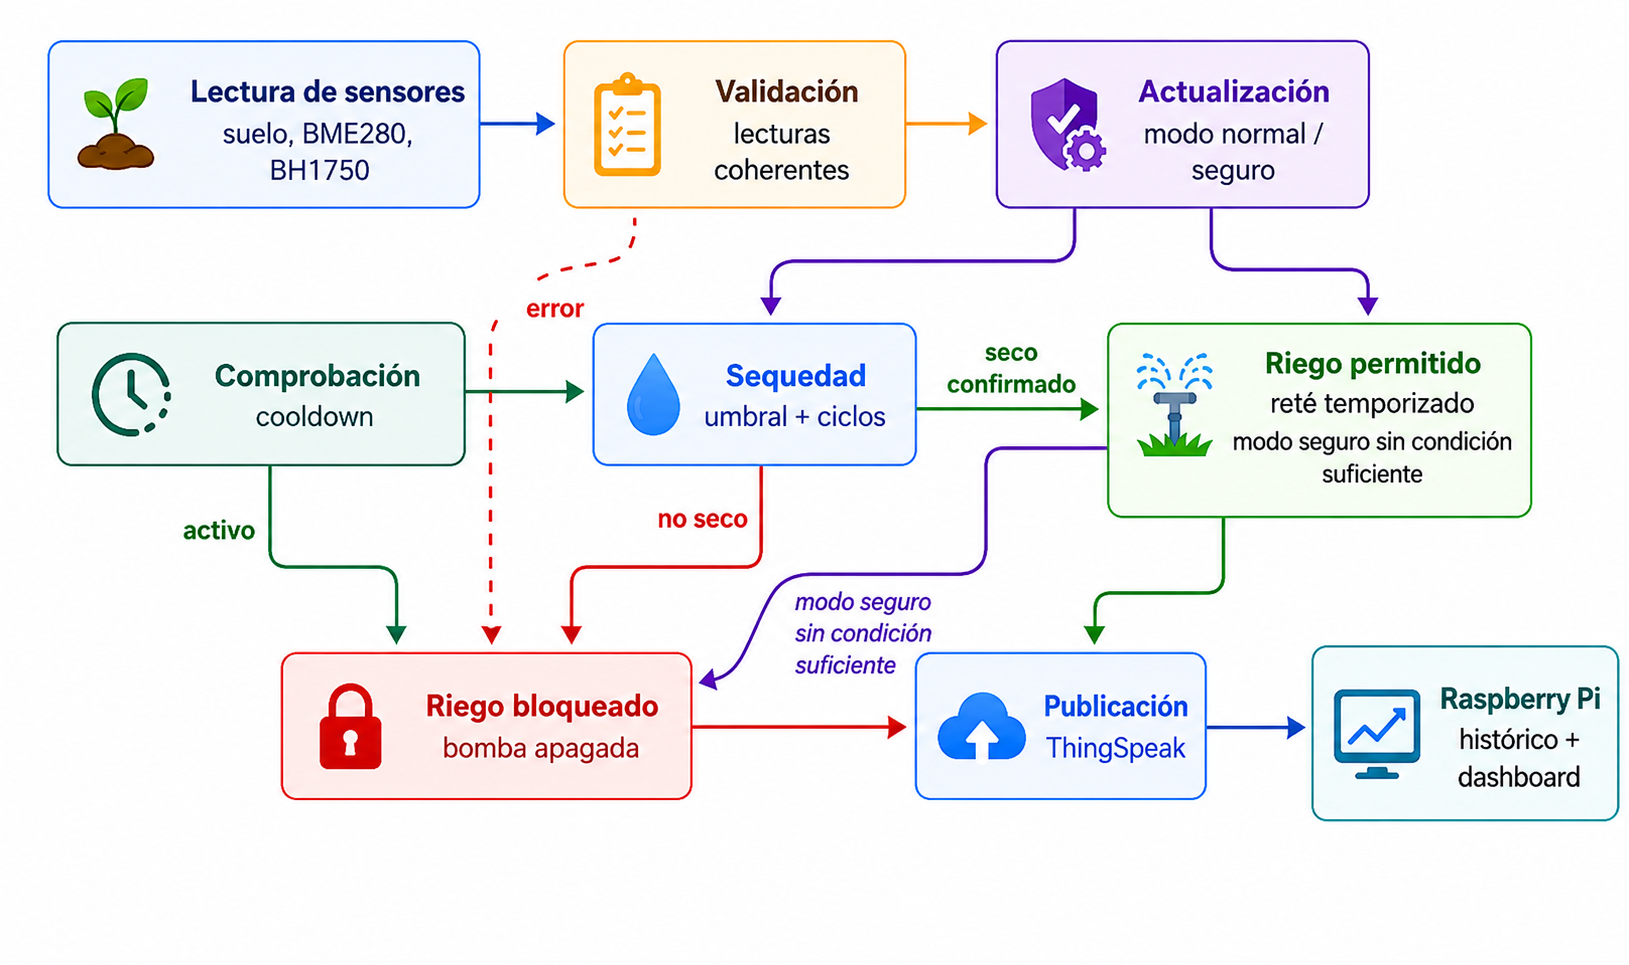
\includegraphics[width=\textwidth]{figs_png/motor_reglas_flujo.png}
\caption{Flujo lógico simplificado de la lógica local de decisión. La estación decide localmente y la Raspberry Pi supervisa el resultado publicado.}
\label{fig:cap6_motor_reglas_flujo}
\end{figure}

El primer filtro de la lógica de decisión es la validez de los sensores. Una lectura ausente, incoherente o no inicializada no debe activar la bomba. Si el firmware detecta un problema en las medidas necesarias para decidir, el sistema adopta una respuesta conservadora: no riega, mantiene el relé apagado y publica el código \texttt{400}. Este código permite que la Raspberry Pi y el dashboard distingan un estado de error de una situación normal sin riego.

El segundo elemento es el modo de funcionamiento. En modo normal, la estación evalúa si la humedad del suelo está por debajo del umbral configurado y si esa condición se mantiene durante los ciclos necesarios. En modo seguro, la estación se comporta de forma más restrictiva: no basta con una lectura puntual de sequedad, sino que se exige una condición más clara antes de permitir la actuación. Si el sistema se encuentra en modo seguro y no se autoriza el riego, se publica el código \texttt{206}.

El tercer elemento es el cooldown. Después de una actuación, la estación espera un tiempo mínimo antes de permitir otro riego. Esta regla evita activaciones repetidas por lecturas inestables o por la lenta estabilización del sensor después de aportar agua. En pruebas de demostración este valor puede configurarse con una duración reducida, por ejemplo decenas de segundos, mientras que en una instalación real debería utilizarse un valor más conservador. Si el cooldown está activo, el sistema no riega y publica el código \texttt{429}.

La decisión de riego se basa principalmente en la humedad del suelo. En la versión actual del firmware, la estación compara el porcentaje de humedad con un umbral normal o con un umbral de modo seguro, según el estado interno. Además, mantiene un contador de ciclos secos consecutivos. Esta confirmación por ciclos evita que una única lectura anómala active la bomba. La Figura~\ref{fig:cap6_confirmacion_humedad} representa esta lógica de forma simplificada.

\begin{figure}[H]
\centering
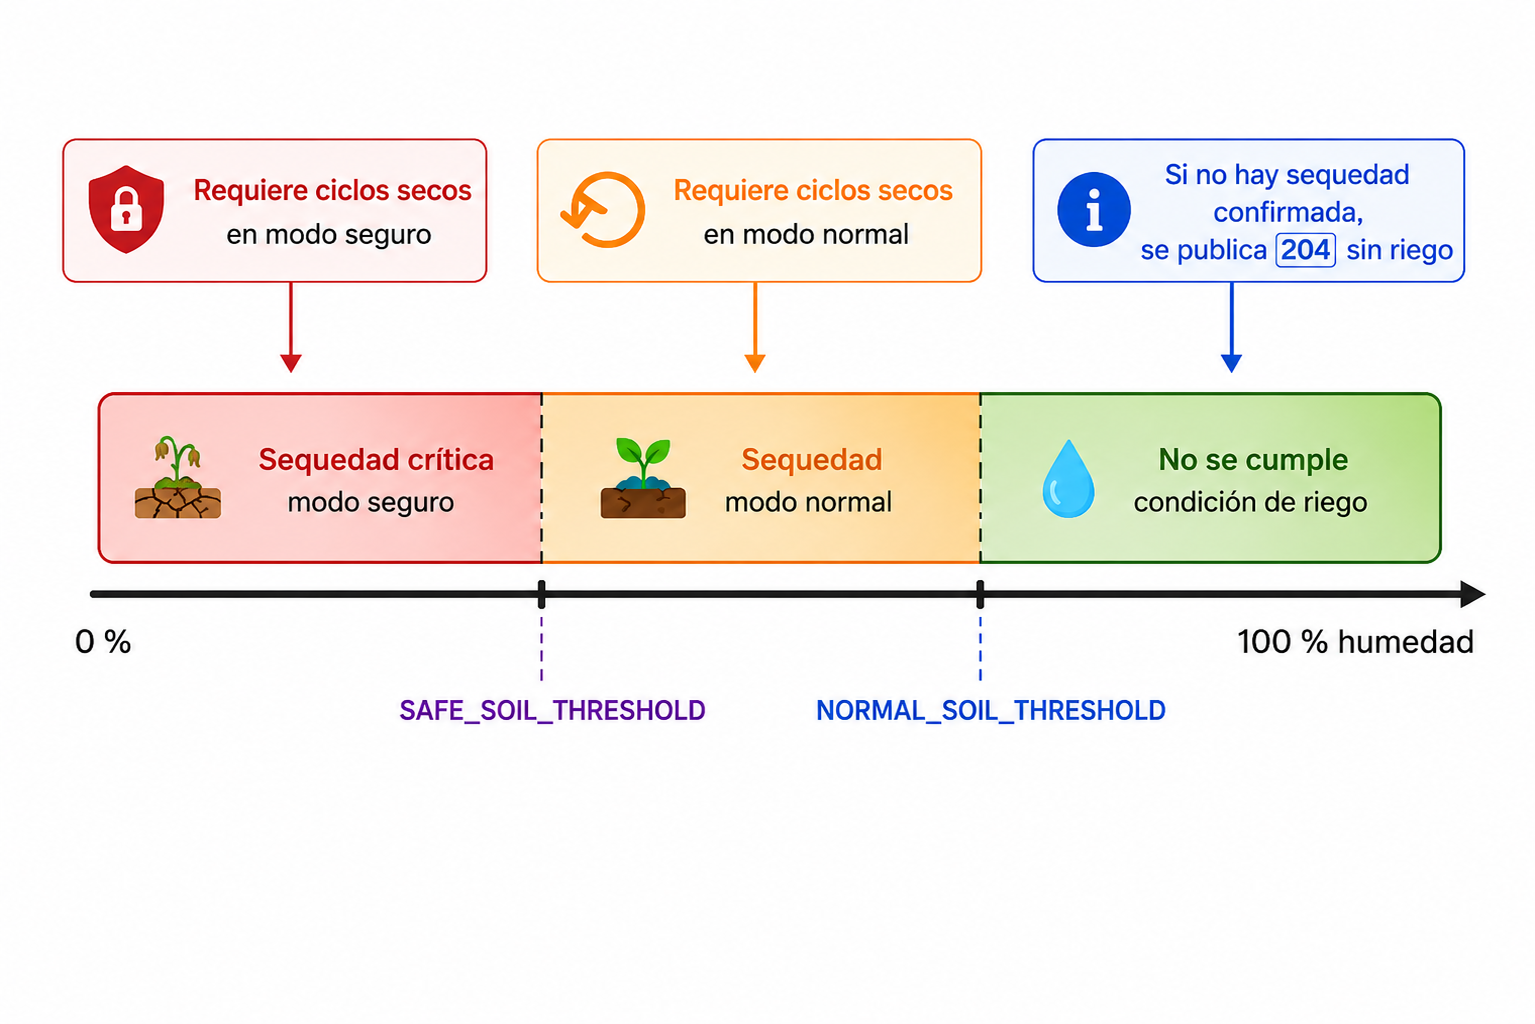
\includegraphics[width=\textwidth]{figs_png/cap6_confirmacion_humedad.png}
\caption{Confirmación de sequedad mediante umbrales y ciclos consecutivos. El modo seguro utiliza una condición más restrictiva que el modo normal.}
\label{fig:cap6_confirmacion_humedad}
\end{figure}

En este contexto, la histéresis no se implementa como un control continuo que mantenga la bomba encendida hasta alcanzar otro umbral. Esto sería menos seguro para el prototipo, porque dependería de que el sensor reaccionase inmediatamente al riego. En TierraViva, la histéresis se aplica de forma práctica mediante tres mecanismos: confirmación por ciclos secos, separación entre umbral normal y umbral de modo seguro, y cooldown después de cada actuación. Así se evita que pequeñas oscilaciones alrededor del umbral provoquen riegos repetidos o cambios de estado demasiado frecuentes.

Cuando el riego se autoriza, la bomba no queda activa indefinidamente. La actuación se ejecuta mediante una función temporizada: se activa el relé, se espera la duración configurada y se desactiva siempre al finalizar. Este comportamiento es esencial porque el apagado de la bomba no depende de la Raspberry Pi, del dashboard ni de una nueva lectura de ThingSpeak. La estación cierra localmente el ciclo de actuación.

La Tabla~\ref{cuadro:cap6_codigos_motor} resume los códigos actuales publicados por la estación. Estos códigos son los que deben interpretarse desde la Raspberry Pi y el dashboard para mostrar el estado operativo de cada estación.

\begin{table}[H]
\centering
\small
\begin{tabular}{|p{0.16\textwidth}|p{0.28\textwidth}|p{0.46\textwidth}|}
\hline
\textbf{Código} & \textbf{Estado} & \textbf{Interpretación} \\
\hline
\texttt{200} & Riego ejecutado / OK & La estación ha autorizado y completado una actuación de riego temporizada. \\
\hline
\texttt{204} & Sin riego & Las lecturas son válidas, pero no se cumple la condición de sequedad confirmada. \\
\hline
\texttt{206} & Modo seguro & La estación se encuentra en modo conservador y no autoriza riego salvo condición suficientemente clara. \\
\hline
\texttt{400} & Error de sensores & Una lectura necesaria no es válida o algún sensor crítico no responde correctamente. \\
\hline
\texttt{429} & Cooldown & Se bloquea una nueva actuación porque no ha transcurrido el tiempo mínimo desde el último riego. \\
\hline
\end{tabular}
\caption{Códigos actuales publicados por la estación.}
\label{cuadro:cap6_codigos_motor}
\end{table}

La lógica principal puede resumirse mediante el fragmento del Código~\ref{cod:motor_reglas_decision}. No se incluye el sketch completo, sino la parte esencial de la decisión. El orden de comprobación es relevante: primero se descartan errores de sensores, después se comprueba el cooldown, y solo entonces se evalúa la sequedad según el modo normal o seguro.

\begin{code}[H]
\begin{lstlisting}[language=C++]
bool shouldIrrigate() {
  if (!sensorOk) {
    statusCode = 400;       // Error de sensores
    return false;
  }

  if (cooldownActive()) {
    statusCode = 429;       // Cooldown activo
    return false;
  }

  if (safeMode) {
    return (soilPercent <= SAFE_SOIL_THRESHOLD) &&
           (dryCycleCount >= SAFE_CONFIRM_DRY_CYCLES);
  }

  return (soilPercent <= NORMAL_SOIL_THRESHOLD) &&
         (dryCycleCount >= NORMAL_CONFIRM_DRY_CYCLES);
}
\end{lstlisting}
\caption{Resumen de la decisión local de riego}
\label{cod:motor_reglas_decision}
\end{code}

El código anterior no asigna por sí solo todos los estados finales. Cuando \texttt{shouldIrrigate()} devuelve \texttt{true}, el bucle principal ejecuta el riego temporizado y publica \texttt{200}. Cuando devuelve \texttt{false}, el firmware distingue la causa: error de sensores, cooldown, modo seguro o ausencia de necesidad de riego. Esta separación permite que el dashboard no muestre simplemente ``riego/no riego'', sino el motivo de la decisión.

\begin{code}[H]
\begin{lstlisting}[language=C++]
readSensors();
updateSafetyState();

if (shouldIrrigate()) {
  irrigateForSeconds(IRRIGATION_SECONDS);
  statusCode = 200;      // Riego ejecutado
} else {
  if (!sensorOk) {
    statusCode = 400;    // Error de sensores
  } else if (cooldownActive()) {
    statusCode = 429;    // Cooldown activo
  } else if (safeMode) {
    statusCode = 206;    // Modo seguro
  } else {
    statusCode = 204;    // Sin riego
  }
}

sendThingSpeak();
\end{lstlisting}
\caption{Asignación del código operativo antes de publicar en ThingSpeak}
\label{cod:asignacion_codigos_motor}
\end{code}

La actuación sobre el relé se limita temporalmente. El firmware activa la salida de control, espera el número de segundos configurado y después apaga el relé. En el montaje real, esta salida controla el módulo de relé que alimenta la bomba de agua de 12 V. La decisión de apagar el relé desde el propio firmware reduce el riesgo de riego indefinido ante fallos de comunicación o pérdida de supervisión.

\begin{code}[H]
\begin{lstlisting}[language=C++]
void irrigateForSeconds(unsigned long seconds) {
  relayActive = true;
  digitalWrite(RELAY_PIN, RELAY_ON);

  delay(seconds * 1000UL);

  digitalWrite(RELAY_PIN, RELAY_OFF);
  relayActive = false;
  lastIrrigationEndMs = millis();
}
\end{lstlisting}
\caption{Actuación temporizada sobre el relé}
\label{cod:riego_temporizado}
\end{code}

El resultado de cada ciclo se publica en ThingSpeak junto con la telemetría. Los campos de sensores permiten interpretar el contexto físico de la estación, mientras que el estado del relé y el código operativo permiten conocer el resultado de la decisión. La Raspberry Pi consulta posteriormente esos datos, los almacena en SQLite y los expone al dashboard, pero no modifica la decisión local tomada por la estación.

Este diseño hace que la lógica local sea simple, verificable y seguro. Simple, porque utiliza condiciones explícitas y parámetros configurables. Verificable, porque cada salida puede relacionarse con un código concreto publicado en ThingSpeak. Y seguro, porque ante lecturas inválidas, cooldown activo o modo seguro no confirmado, la respuesta por defecto es mantener la bomba apagada. De este modo, TierraViva cierra localmente el ciclo medir--decidir--actuar, mientras que la Raspberry Pi conserva el papel de supervisión e histórico.

\section{API FastAPI}
\label{sec:api_fastapi}

La API de TierraViva constituye la capa de servicio entre la base de datos local y el dashboard web. Su función no es comunicarse directamente con las estaciones ni decidir el riego, sino ofrecer una interfaz HTTP para consultar de forma estructurada la información ya almacenada en la Raspberry Pi. De este modo, el frontend no necesita acceder directamente a SQLite ni conocer los detalles internos del módulo de ingesta.

\begin{wrapfigure}{r}{0.32\textwidth}
    \vspace{-12pt}
    \centering
    
\includegraphics[width=0.30\textwidth]{figs/fast_api_logo.png}
    \caption{Logo FastAPI}
    \label{fig:logo_fastapi}
    \vspace{-8pt}
\end{wrapfigure}

La implementación se realiza con FastAPI, un framework Python orientado a la creación de APIs web. En el contexto de TierraViva, FastAPI permite definir endpoints claros, validar parámetros de consulta y devolver respuestas en formato JSON. Esta elección mantiene el código compacto, facilita la depuración y ofrece una documentación automática de la API durante la ejecución del servidor.

La API se ejecuta mediante Uvicorn, escuchando en el puerto \texttt{8000}. El script de gestión \texttt{tierraviva.sh} arranca por separado el proceso de ingesta y el servidor web, de modo que la lectura de ThingSpeak y la consulta desde el dashboard quedan desacopladas. Si el dashboard realiza varias peticiones seguidas, estas se atienden desde la base de datos local, sin forzar una consulta nueva a ThingSpeak en cada refresco de pantalla.

La Figura~\ref{fig:cap6_api_flujo} resume el papel de la API dentro del software de la Raspberry Pi.

\begin{figure}[H]
\centering
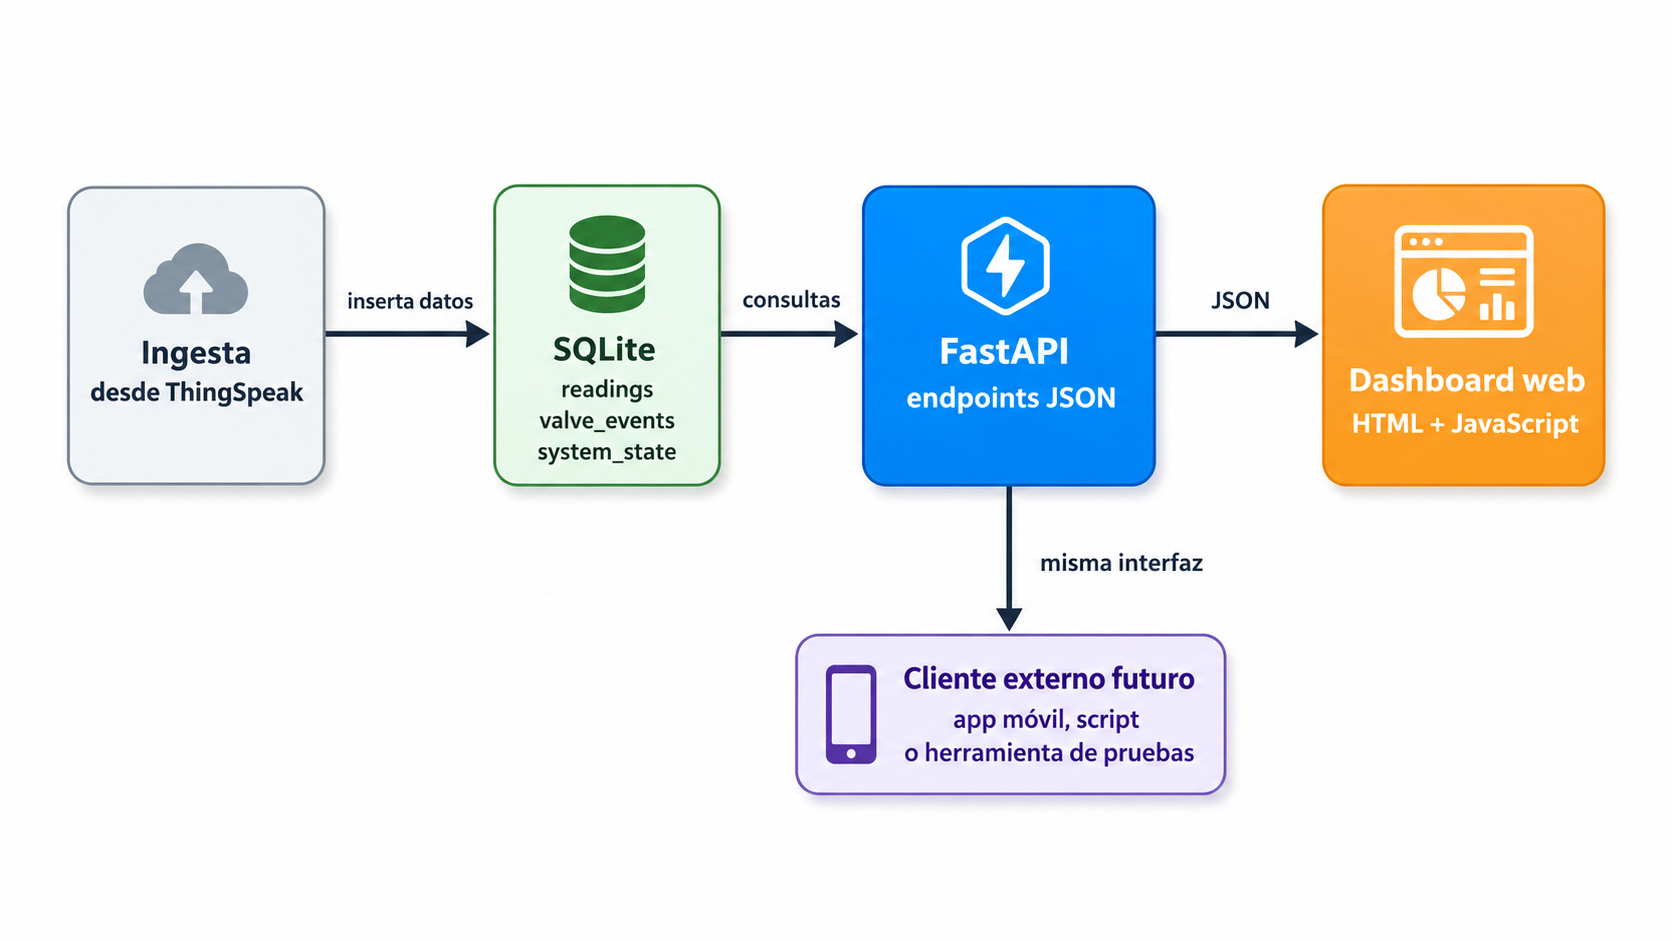
\includegraphics[width=0.80\textwidth]{figs_png/api_flujo.png}
\caption{Papel de FastAPI como capa de servicio entre SQLite y los clientes de consulta.}
\label{fig:cap6_api_flujo}
\end{figure}

El diseño de la API sigue una separación de responsabilidades sencilla. El módulo \texttt{database.py} conserva las funciones de acceso a datos; \texttt{api.py} se limita a validar parámetros, llamar a esas funciones y enriquecer algunas respuestas con información útil para la interfaz. Por ejemplo, una lectura puede completarse con su antigüedad en segundos, una etiqueta de frescura y una clasificación del estado del suelo.

La Tabla~\ref{cuadro:cap6_endpoints_api} resume los endpoints principales de la API. 

\begin{table}[H]
\centering
\small
\setlength{\tabcolsep}{4pt}
\renewcommand{\arraystretch}{1.1}
\begin{tabular}{|p{0.27\textwidth}|p{0.15\textwidth}|p{0.48\textwidth}|}
\hline
\textbf{Endpoint} & \textbf{Método} & \textbf{Función principal} \\
\hline
\texttt{/} & GET & Sirve el fichero \texttt{index.html} del dashboard. \\
\hline
\texttt{/api/config} & GET & Devuelve la configuración general del sistema: estación seleccionada, estaciones activas, umbrales, ruta de base de datos y últimas marcas de ingesta. \\
\hline
\texttt{/api/latest} & GET & Devuelve la última lectura almacenada para una estación, junto con antigüedad, frescura y estado interpretado del suelo. \\
\hline
\texttt{/api/readings} & GET & Devuelve el histórico reciente de lecturas de una estación, con un límite configurable de muestras. \\
\hline
\texttt{/api/stats} & GET & Calcula estadísticas agregadas para una ventana temporal configurable. \\
\hline
\texttt{/api/health} & GET & Comprueba el estado básico del servicio: base de datos, frontend y disponibilidad de lecturas. \\
\hline
\end{tabular}
\caption{Endpoints implementados en la API FastAPI}
\label{cuadro:cap6_endpoints_api}
\end{table}

El endpoint \texttt{/api/latest} se utiliza para obtener la situación más reciente de una estación. Recibe como parámetro el identificador de estación, por ejemplo \texttt{station=A}, y devuelve la última lectura almacenada. Además de los datos originales, la API calcula campos derivados como \texttt{age\_seconds}, \texttt{freshness} y \texttt{soil\_state}. Estos campos evitan que el dashboard tenga que repetir lógica de interpretación en JavaScript.

\begin{lstlisting}[language=Python, caption={Esquema simplificado del endpoint de última lectura}, label={cod:api_latest}]
@app.get("/api/latest")
def api_latest(station: Optional[str] = Query(None)):
    selected_station = normalize_station(station)
    reading = get_latest_reading(selected_station)

    if reading is None:
        return {
            "ok": False,
            "station": selected_station,
            "reading": None,
            "status": "sin_datos",
        }

    age_seconds = age_seconds_from_ts(reading["ts"])
    soil = reading.get("soil_moisture_pct")

    return {
        "ok": True,
        "station": selected_station,
        "reading": reading,
        "age_seconds": age_seconds,
        "freshness": freshness_label(age_seconds),
        "soil_state": soil_label(soil),
    }
\end{lstlisting}

El endpoint \texttt{/api/readings} expone el histórico reciente. Su parámetro \texttt{limit} permite controlar cuántas muestras se devuelven, con límites internos para evitar respuestas excesivamente grandes. Esta consulta es la base de las gráficas temporales del dashboard, ya que permite recuperar las últimas medidas de humedad del suelo, temperatura, humedad relativa, luminosidad y presión.

El endpoint \texttt{/api/stats} proporciona un resumen agregado para una ventana temporal expresada en horas. Con \texttt{hours=24} se obtiene un resumen diario; con \texttt{hours=168}, un resumen semanal. Esta decisión evita crear endpoints separados para día y semana, y permite reutilizar la misma función para diferentes escalas temporales. El resultado puede incluir valores medios, mínimos y máximos de las principales magnitudes registradas.

\begin{table}[H]
\centering
\small
\begin{tabular}{|p{0.30\textwidth}|p{0.25\textwidth}|p{0.35\textwidth}|}
\hline
\textbf{Consulta} & \textbf{Ejemplo} & \textbf{Uso en el sistema} \\
\hline
Última lectura de A & \texttt{/api/latest?station=A} & Tarjetas principales del dashboard. \\
\hline
Histórico reciente de B & \texttt{/api/readings?station=B\&limit=120} & Gráficas de evolución temporal. \\
\hline
Resumen diario & \texttt{/api/stats?station=A\&hours=24} & Valores medios, mínimos y máximos del último día. \\
\hline
Resumen semanal & \texttt{/api/stats?station=A\&hours=168} & Análisis de tendencia semanal. \\
\hline
Consulta de salud & \texttt{/api/health?station=A} & Diagnóstico básico del servicio, disponibilidad de datos y existencia del frontend. \\
\hline
Configuración de A & \texttt{/api/config?station=A} & Consulta de umbrales, estación activa, rutas locales y última ingesta registrada. \\
\hline
\end{tabular}
\caption{Ejemplos de consulta a la API}
\label{cuadro:cap6_consultas_api}
\end{table}

La API pública se mantiene deliberadamente centrada en la consulta de lecturas, configuración, estadísticas y diagnóstico. Aunque la base de datos contiene una tabla preparada para eventos operativos, la versión actual del backend no expone endpoints de control ni de envío de órdenes hacia las estaciones. Esta decisión mantiene la coherencia con la arquitectura final: la Raspberry Pi consulta y muestra información, pero no participa en la actuación física sobre el riego.

Desde el punto de vista del dashboard, esta API permite construir una interfaz reactiva sin acoplarla a la base de datos. La web puede solicitar periódicamente \texttt{/api/latest}, \texttt{/api/readings} y \texttt{/api/stats}; si una estación deja de actualizarse, la antigüedad de la última lectura permite mostrar un estado \textit{fresh}, \textit{stale} u \textit{offline}. Esta lógica mejora la interpretación visual: no basta con enseñar el último valor recibido, también es necesario indicar si ese valor sigue siendo reciente.

El endpoint \texttt{/api/health} se reserva para diagnóstico. Devuelve información básica sobre el servicio, como la existencia del frontend, la ruta de la base de datos y si hay datos disponibles para alguna estación. Este tipo de endpoint es útil durante la instalación en Raspberry Pi, porque permite comprobar rápidamente si el servidor está levantado y si la API puede acceder a la información local.

En conjunto, FastAPI actúa como una frontera clara entre almacenamiento y visualización. La base de datos conserva el histórico; la API lo transforma en respuestas JSON coherentes; y el dashboard consume esas respuestas sin conocer la estructura interna de SQLite. Esta separación hace que el software sea más mantenible y deja abierta la posibilidad de añadir otros clientes en el futuro, como una aplicación móvil, una herramienta de análisis o scripts de validación, reutilizando la misma interfaz HTTP.

\section{Dashboard web de supervisión}
\label{sec:dashboard_web_supervision}

El último bloque software de la Raspberry Pi es el dashboard web de supervisión. Su función es presentar al usuario la información almacenada y servida por la API de forma comprensible, sin obligarle a consultar directamente ThingSpeak, SQLite o los logs del sistema. El dashboard no participa en la decisión de riego ni envía órdenes a las estaciones; actúa como interfaz de visualización del estado publicado por los nodos de campo.

La interfaz principal se define en el fichero \texttt{dashboard/index.html}, mientras que la lógica de actualización se implementa en \texttt{dashboard/js/tierraviva.js}. El fichero HTML contiene la estructura visual del panel: cabecera, selector de estación, tarjetas de lectura actual, gráficas, resumen histórico y tabla de últimas lecturas. El fichero JavaScript se encarga de consultar periódicamente la API, interpretar las respuestas y actualizar los elementos de la página.

El dashboard está organizado alrededor de una estación seleccionada. En la versión actual se contemplan las estaciones \texttt{A} y \texttt{B}, y el usuario puede alternar entre ellas mediante un selector. Esta decisión mantiene la coherencia con la arquitectura multiestación del sistema: la misma interfaz puede mostrar datos de distintas zonas sin duplicar el código del frontend.

La Tabla~\ref{cuadro:cap6_campos_dashboard} resume los principales campos mostrados en el dashboard.

\begin{table}[H]
\centering
\small
\begin{tabular}{|p{0.28\textwidth}|p{0.30\textwidth}|p{0.32\textwidth}|}
\hline
\textbf{Elemento mostrado} & \textbf{Origen en la API} & \textbf{Interpretación} \\
\hline
Humedad del suelo & \texttt{soil\_moisture\_pct} & Valor normalizado de humedad utilizado para clasificar el suelo como seco, normal o húmedo. \\
\hline
Temperatura & \texttt{temperature\_c} & Temperatura ambiente medida por la estación. \\
\hline
Humedad ambiental & \texttt{humidity\_pct} & Humedad relativa del aire. \\
\hline
Luminosidad & \texttt{light\_lux} & Nivel de luz ambiente medido en lux. \\
\hline
Presión & \texttt{pressure\_hpa} & Presión atmosférica medida por el sensor ambiental. \\
\hline
Última lectura & \texttt{ts}, \texttt{age\_seconds}, \texttt{freshness} & Información temporal para saber si los datos son recientes, antiguos u obsoletos. \\
\hline
Estado del relé & \texttt{relay\_state} & Indica si el bloque de actuación aparece como apagado o activo según la última publicación. \\
\hline
Estado/evento & \texttt{system\_event} & Estado operativo publicado por la estación. \\
\hline
Debug/código & \texttt{debug\_code} & Código auxiliar de diagnóstico o estado publicado por la estación. \\
\hline
\end{tabular}
\caption{Campos principales mostrados en el dashboard web}
\label{cuadro:cap6_campos_dashboard}
\end{table}

La pantalla inicial muestra tarjetas con las magnitudes más recientes: humedad del suelo, temperatura, humedad ambiental, luminosidad y presión. Estas tarjetas permiten comprobar rápidamente el estado de la estación seleccionada. Además, el panel incluye información de actualización, mostrando si la última lectura se considera reciente, retrasada u obsoleta. Esta distinción es importante porque un valor aparentemente correcto puede no ser útil si la estación lleva demasiado tiempo sin publicar datos nuevos.

El dashboard también interpreta la humedad del suelo mediante umbrales configurados. En lugar de mostrar únicamente un número, el frontend clasifica el valor como \textit{seco}, \textit{normal} o \textit{húmedo}. Esta interpretación se realiza a partir de los umbrales recibidos desde \texttt{/api/config}. De esta forma, la interfaz puede adaptarse a cambios de configuración sin modificar manualmente el código HTML.

La actualización de datos se realiza mediante peticiones HTTP periódicas a la API. El script \texttt{tierraviva.js} consulta los endpoints \texttt{/api/config}, \texttt{/api/latest}, \texttt{/api/readings} y \texttt{/api/stats} para obtener configuración, última lectura, histórico reciente y resumen estadístico. Estas peticiones se realizan para la estación seleccionada, utilizando el parámetro \texttt{station}. El intervalo de refresco se obtiene de la configuración del sistema mediante \texttt{web\_refresh\_seconds}; si no está disponible, se utiliza un valor por defecto de tres segundos.

\begin{table}[H]
\centering
\small
\begin{tabular}{|p{0.42\textwidth}|p{0.50\textwidth}|}
\hline
\textbf{Consulta realizada por el dashboard} & \textbf{Uso en la interfaz} \\
\hline
\texttt{/api/config?station=A} & Obtener estación activa, lista de estaciones, umbrales y periodo de refresco. \\
\hline
\texttt{/api/latest?station=A} & Actualizar las tarjetas principales con la última lectura disponible. \\
\hline
\texttt{/api/readings?station=A\&limit=10} & Construir gráficas y tabla de lecturas recientes. \\
\hline
\texttt{/api/stats?station=A\&hours=24} & Mostrar el resumen histórico de las últimas 24 horas. \\
\hline
\end{tabular}
\caption{Consultas principales realizadas por el dashboard a la API}
\label{cuadro:cap6_consultas_dashboard}
\end{table}

Además de las tarjetas principales, el dashboard incorpora gráficas de evolución temporal. Estas gráficas permiten observar la tendencia reciente de las variables ambientales y de suelo, en lugar de analizar únicamente la última muestra recibida. Esta visualización resulta útil durante las pruebas porque permite detectar comportamientos anómalos, valores constantes, saltos bruscos o ausencia de actualización.

El panel incluye también un resumen histórico de las últimas 24 horas. Este resumen calcula valores agregados, como medias, mínimos y máximos, a partir de los datos devueltos por la API. En el caso de los campos operativos, como el estado del relé, el estado/evento y el código de depuración, el dashboard muestra información de frecuencia o último valor disponible. Así, el usuario puede distinguir no solo las condiciones ambientales, sino también el comportamiento operativo reciente de la estación.

La tabla de últimas lecturas completa la visualización. En ella se muestran varias muestras recientes con fecha, humedad del suelo, temperatura, humedad relativa, luminosidad y presión. Esta tabla resulta especialmente útil durante la depuración, ya que permite comprobar si las lecturas se insertan en orden, si aparecen valores nulos o si la evolución de los datos es coherente con lo mostrado en las tarjetas y gráficas.

Desde el punto de vista de diseño, el dashboard se mantiene como una capa de presentación. No accede directamente a ThingSpeak ni a SQLite, sino que consume exclusivamente la API expuesta por FastAPI. Esta separación evita duplicar lógica de acceso a datos en el frontend y facilita que los cambios en la base de datos o en la ingesta no obliguen a modificar la estructura visual, siempre que la API mantenga el contrato de respuesta.

En caso de error, ausencia de datos o pérdida de actualización, el dashboard no debe ocultar la situación. Si la API no devuelve una lectura válida, la interfaz muestra valores vacíos o mensajes de espera. Si la lectura existe pero es antigua, el estado de frescura permite indicar que la estación no se está actualizando correctamente. Esta forma de visualización es importante en TierraViva porque la supervisión no consiste solo en mostrar números, sino en informar de si esos números siguen siendo fiables.

En conjunto, el dashboard web convierte los datos técnicos del sistema en una vista útil para el usuario. Las estaciones siguen siendo responsables de medir, decidir y actuar localmente; la Raspberry conserva el histórico y sirve la API; y el dashboard permite supervisar el estado del sistema sin intervenir en la actuación física. Con ello se cierra el flujo software de TierraViva: ingesta desde ThingSpeak, almacenamiento en SQLite, exposición mediante FastAPI y visualización web.

\section{Ejecución y gestión del sistema software}
\label{sec:ejecucion_gestion_software}

Para facilitar la puesta en marcha del software en la Raspberry Pi, el proyecto incluye el script \texttt{tierraviva.sh}. Este script agrupa las operaciones principales de despliegue y ejecución, evitando tener que lanzar manualmente cada componente desde la terminal.

El script permite instalar dependencias, preparar el entorno virtual, copiar el dashboard al directorio esperado por FastAPI, arrancar el proceso de ingesta \texttt{main.py}, iniciar el servidor \texttt{api.py} mediante Uvicorn, consultar el estado de ejecución, detener los procesos y revisar los logs. Esta automatización resulta útil durante las pruebas porque reduce errores repetitivos de arranque y deja una forma reproducible de iniciar el sistema.

\begin{table}[H]
\centering
\small
\begin{tabular}{|p{0.25\textwidth}|p{0.60\textwidth}|}
\hline
\textbf{Comando} & \textbf{Función} \\
\hline
\texttt{./tierraviva.sh install} & Crea el entorno, instala dependencias e inicializa la base de datos. \\
\hline
\texttt{./tierraviva.sh start} & Arranca el proceso de ingesta y el servidor de la API, mostrando los logs. \\
\hline
\texttt{./tierraviva.sh stop} & Detiene los procesos asociados al sistema. \\
\hline
\texttt{./tierraviva.sh restart} & Reinicia los servicios del prototipo. \\
\hline
\texttt{./tierraviva.sh status} & Muestra si \texttt{main.py} y \texttt{api.py} están en ejecución. \\
\hline
\texttt{./tierraviva.sh logs} & Muestra las últimas líneas de log generadas por los procesos. \\
\hline
\end{tabular}
\caption{Operaciones principales del script de gestión \texttt{tierraviva.sh}}
\label{cuadro:cap6_tierraviva_sh}
\end{table}

Además de arrancar los procesos, el script carga el fichero \texttt{.env} cuando está disponible. Esto permite mantener fuera del código fuente las claves de ThingSpeak y los identificadores de canal. Durante el arranque, el script comprueba que existen las variables necesarias para consultar las estaciones configuradas, como los identificadores de canal y las claves de lectura de ThingSpeak. Si faltan identificadores de canal o claves de lectura, el proceso de ingesta no continúa como si el sistema estuviera correctamente configurado, sino que deja el error reflejado en los logs.

Esta capa de gestión no modifica la arquitectura del sistema: la estación sigue siendo autónoma y la Raspberry mantiene un papel de supervisión. Su valor está en hacer que el backend sea más reproducible, más fácil de ejecutar y más sencillo de depurar durante las pruebas.

